\chapter{Generative and Performative Algorithms}

\section{Introduction}

Today, two main paradigms of algorithmic design are clearly dominant; generative design and performative design \cite{fasoulaki08}. Generative design is the essential \emph{rule-based} algorithmic form of digital architecture. It is governed by repitive patterns, equations and shape transformations.  Performative design on the other hand, is optimizational; modifing and reshaping to adapt to a certain simulated environment.

\section{Generative Design}

Generative architecture can be defined as a design process involving generative systems in the form of a computar program that can be fully automated or step-by-step controlled. It would have an algorithm (rule) governing the transformations of initial shapes through variables or parameters; `generating' results, and selecting the best variant according to the given criteria. \cite{arida04}

\subsection{Generative Systems}

The tools and key components of generative design are the systems which define the method of form exploration. They can be defined as scripts or sets of geometrical transformations \cite{arida04}. These systems ---as mentioned earlier--- are rule based, essentially formal or visual and are often based on systems borrowed from biology and mathematics. Some popular systems widely used today include Cellular Automata, L-Systems, Voronoi Diagrams, Fractals and Shape Grammars.

\subsubsection{Cellular Automata}

``Cellular Automata is a computational method which can simulate the process of growth by describing a complex system by simple individuals following simple rules. The concept of simulating growth was introduced by John von Neumann (1951) and further developed by Ulam (1962) in the are of simulating multi-state machines. The concept gained great popularity when Martin Gardner (1970) John Conway's ``Life'', a game that generated two dimensional patterns''\cite{krawczyk02}. Later on, Stephen Wolfram would begin reserch on the subject in 1984, to write a book on the subject called \emph{A New Kind of Science} \cite{wolfram02}. The book would discuss the patterns created by cellular automata as simple rules capable of generating extremely complex patterns that mimic patterns of growth occuring in nature, among other things; describing his findings as a new paradigm of scientific research touching on numerous fields of science.

\begin{figure}[htbp]
\centering
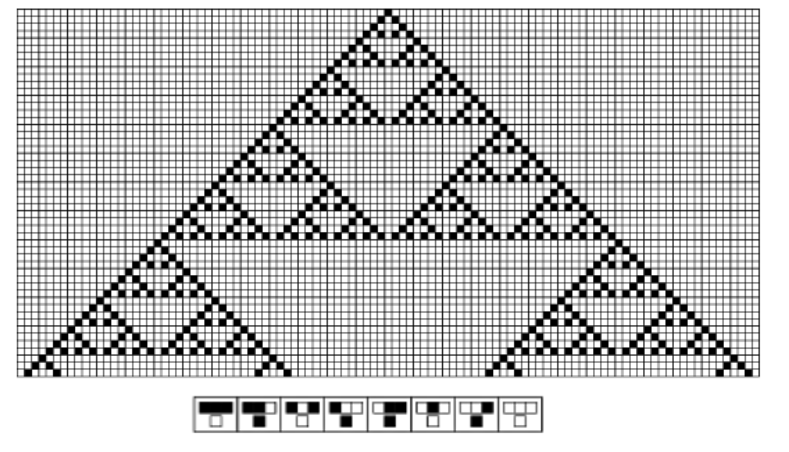
\includegraphics[width=\textwidth]{./Images/1-CellAutoEg}
\caption[Cellular Automaton]{An example of cellular automata showing the sequence of generations and the governing rule.\cite{wolfram02}}
\label{CAEg}
\end{figure}

The concept of cellular automata is that an initial configuration of at least one cell occupying an empty space would evolve and procreate into a pattern using a rule that decides birth, life and death cells through the preceding related cells (Fig. \ref{CAEg}). The pattern shown is a two dimensional growth pattern used by Stephen Wolfram. Other forms of cellular automata generation include 3-dimensional ones, which are the architects main interest.

The method of generation in 3-dimensional cellular automata remains basically the same as with 2-dimensional ones; with an initial configuration of blocks occuping spaces and a rule that governs the shape of each generation (Fig \ref{3dCA}).

\begin{figure}[htbp]
\centering
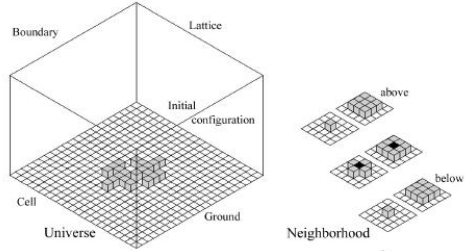
\includegraphics[width=0.7\textwidth]{./Images/2-3dCA}
\caption[3-Dimensional Cellular Automata]{3-Dimensional cellular automata and terminology.\cite{krawczyk02}}
\label{3dCA}
\end{figure}

The utilisation of basic rules of cellular automata however does not suffice to produce architecturally sound models with appropriate internal spaces in most cases (Fig \ref{3dCAArch}). In order to produce such forms, a degree of optimization and modification is required. A fairly simple but effective solution is manipulation of cell interpretation. Examples of such manipulation are stretching cells to overlap forming adequate in ternal spaces, merging the overlapping cells and interpreting the envelope of merged cells as splines (Fig \ref{CA Optimisation}).

\begin{figure}[htbp]
\centering
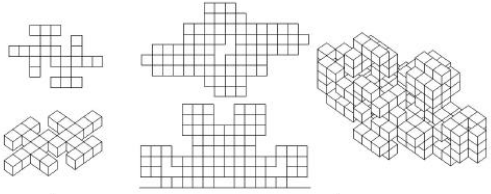
\includegraphics[width=0.5\textwidth]{./Images/3-3dCAArch}
\caption[Cellular Automata Architectural Inadequacy]{An example of CA rules inadequacy for architectural forms without modification \cite{krawczyk02}}
\label{3dCAArch}
\end{figure}


\begin{figure}[htbp]
\centering
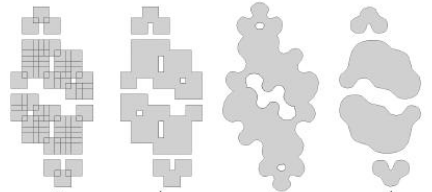
\includegraphics[width=0.7\textwidth]{./Images/4-3dCAArchOpt}
\caption[Cellular Automata Architectural Optimization]{Optimisation of cell interpretation for architectural form \cite{krawczyk02}}
\label{CA Optimisation}
\end{figure}
